% ==============================================================================
% Academic Poster Template — Columbia University
% Size: 36 in (W) × 48 in (H), Portrait, Two Columns
% Engine: LuaLaTeX + beamerposter
% ==============================================================================
\documentclass[final]{beamer}

\usepackage[
  size=custom,
  width=91.44,    % 36 inches in cm
  height=121.92,  % 48 inches in cm
  scale=1.5
]{beamerposter}
% \usepackage[
%   size=A0,
%   orientation=portrait,
%   scale=1.4
% ]{beamerposter}

\usepackage{fontspec}
\usefonttheme{serif}
\setmainfont{Georgia}
\usepackage{amsmath,amssymb}
\usepackage{graphicx}
\usepackage{booktabs}
\usepackage{tikz}
\usepackage{pgfplots}
\usepackage{xcolor}
\usepackage{ragged2e}
\usepackage{array}
\usepackage{microtype}
\usepackage{svg}
\usepackage{caption}
\captionsetup{margin=0.8em}

\setbeamertemplate{navigation symbols}{}

% ------------------------------------------------------------------------------
% Columbia University Colors
% ------------------------------------------------------------------------------
\definecolor{CUNavy}{HTML}{003366}
\definecolor{CUBlue}{HTML}{75AADB}
\definecolor{CULightBlue}{HTML}{D6E8F5}
\definecolor{CUGold}{HTML}{C4B080}
\definecolor{blockbg}{HTML}{F4F8FC}

% ------------------------------------------------------------------------------
% Beamer color / font setup
% ------------------------------------------------------------------------------
\setbeamercolor{background canvas}{bg=white}
\setbeamercolor{normal text}{fg=black}

\setbeamercolor{block title}{fg=white, bg=CUNavy}
\setbeamercolor{block body} {fg=black, bg=blockbg}
\setbeamerfont{block title}{size=\large, series=\bfseries}
\setbeamerfont{block body} {size=\small}

\setbeamercolor{block alerted title}{fg=white, bg=CUGold!75!black}
\setbeamercolor{block alerted body} {fg=black, bg=CUGold!10}
\setbeamerfont{block alerted title}{size=\large, series=\bfseries}

\setbeamertemplate{block begin}{
  \begin{beamercolorbox}[
      rounded=false, ht=2.8ex, dp=1.2ex,
      leftskip=0.8em, rightskip=0.8em
    ]{block title}
    \usebeamerfont{block title}\insertblocktitle
  \end{beamercolorbox}
  \nointerlineskip
  \begin{beamercolorbox}[rounded=false, sep=0.8em]{block body}
  \usebeamerfont{block body}\justifying\setlength\leftskip{0.8em}\setlength\rightskip{0.8em}%
  \noindent\ignorespaces
}
\setbeamertemplate{block end}{\end{beamercolorbox}\vspace{10pt}}

\setbeamertemplate{block alerted begin}{
  \begin{beamercolorbox}[
      rounded=false, ht=2.8ex, dp=1.2ex,
      leftskip=0.8em, rightskip=0.8em
    ]{block alerted title}
    \usebeamerfont{block alerted title}\insertblocktitle
  \end{beamercolorbox}
  \nointerlineskip
  \begin{beamercolorbox}[rounded=false, sep=0.8em]{block alerted body}
  \usebeamerfont{block body}\justifying\setlength\leftskip{0.8em}\setlength\rightskip{0.8em}%
  \noindent\ignorespaces
}
\setbeamertemplate{block alerted end}{\end{beamercolorbox}\vspace{10pt}}

% ==============================================================================
% DOCUMENT
% ==============================================================================
\begin{document}
\begin{frame}{}

% ==============================================================================
% HEADER — navy banner drawn as overlay, column holds actual content
% ==============================================================================
\begin{tikzpicture}[remember picture, overlay]
  \fill[CULightBlue] (-1cm,5cm) rectangle (95cm,-16cm);
  \fill[CUGold] (-1cm,-16cm) rectangle (95cm,-17.5cm);
\end{tikzpicture}

\begin{columns}[T, totalwidth=0.9\paperwidth]
  \begin{column}{0.01\paperwidth}
  \end{column}
  \begin{column}{0.62\paperwidth}\raggedright
    {\color{black}\fontsize{70}{50}\bfseries\selectfont
      XTRACT: The Measurement of Krypton in Xenon with ppq Sensitivity} \\[1.0cm]
    {\color{black}\fontsize{40}{25}\selectfont
      Dacheng~Xu,\;
      Elena~Aprile,\;
      Michael~Murra,\;
      Guillaume~Plante,\;
      George~Stouraitis,\;
      Zihao~Xu} \\[0.5cm]
    {\color{black}\fontsize{30}{25}\selectfont
      \textit{Physics Department, Columbia University, New York, NY 10027, USA}} \\[0.5cm]
    dacheng.xu@columbia.edu \\
  \end{column}
  \begin{column}{0.02\paperwidth}
  \end{column}
  \begin{column}{0.25\paperwidth}\vspace{4.0cm}
    \includesvg[width=30cm]{cu-blue-logo.svg}
  \end{column}
\end{columns}
\begin{columns}[T, totalwidth=0.9\paperwidth]
  \begin{column}{0.01\paperwidth}
  \end{column}
  \begin{column}{0.89\paperwidth}\vspace{2.0cm}
    {\color{black}\fontsize{35}{25}\selectfont
      XeSAT 2026 - International Workshop on Applications of Noble Gas Xenon to Science and Technology}
  \end{column}
\end{columns}
\vspace{2.5cm}

% ==============================================================================
% BODY — two columns, content sized to fill the page height
% ==============================================================================
\begin{columns}[T, totalwidth=\linewidth]

% ============================================================
% LEFT COLUMN
% ============================================================
\begin{column}{0.48\linewidth}

\begin{block}{Motivation: $\boldsymbol{^{85}}$Kr Background}
  $\boldsymbol{^{85}}$Kr is an important contributor to the electronic-recoil background in liquid-xenon dark matter search experiments. It undergoes $\boldsymbol{\beta}$ decay with a Q-value of 687.0~keV~\cite{XENON:2022ltv,LZ:2025zpw,PandaX:2024jjs}. Due to its 10.7-year half-life, the current atmospheric inventory of $\boldsymbol{^{85}}$Kr is predominantly anthropogenic, mainly originating from nuclear fuel reprocessing and nuclear weapons testing.

  \vspace{16pt}
  \begin{center}
    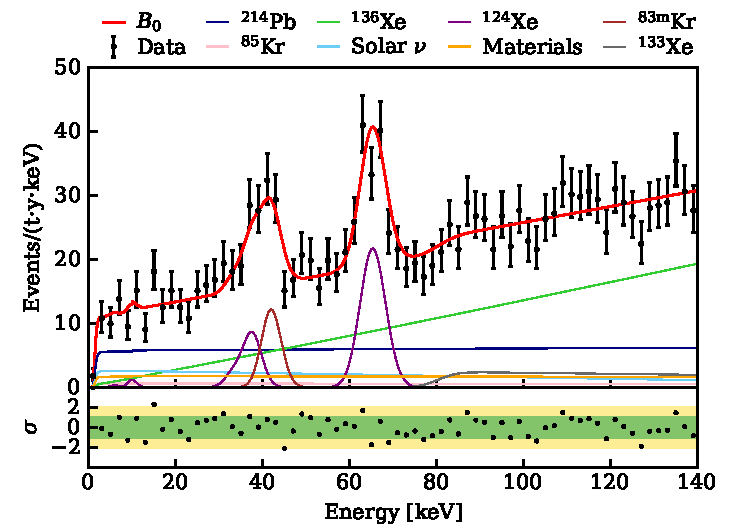
\includegraphics[width=0.51\linewidth]{bkg_only_full_energy.pdf}\hfill
    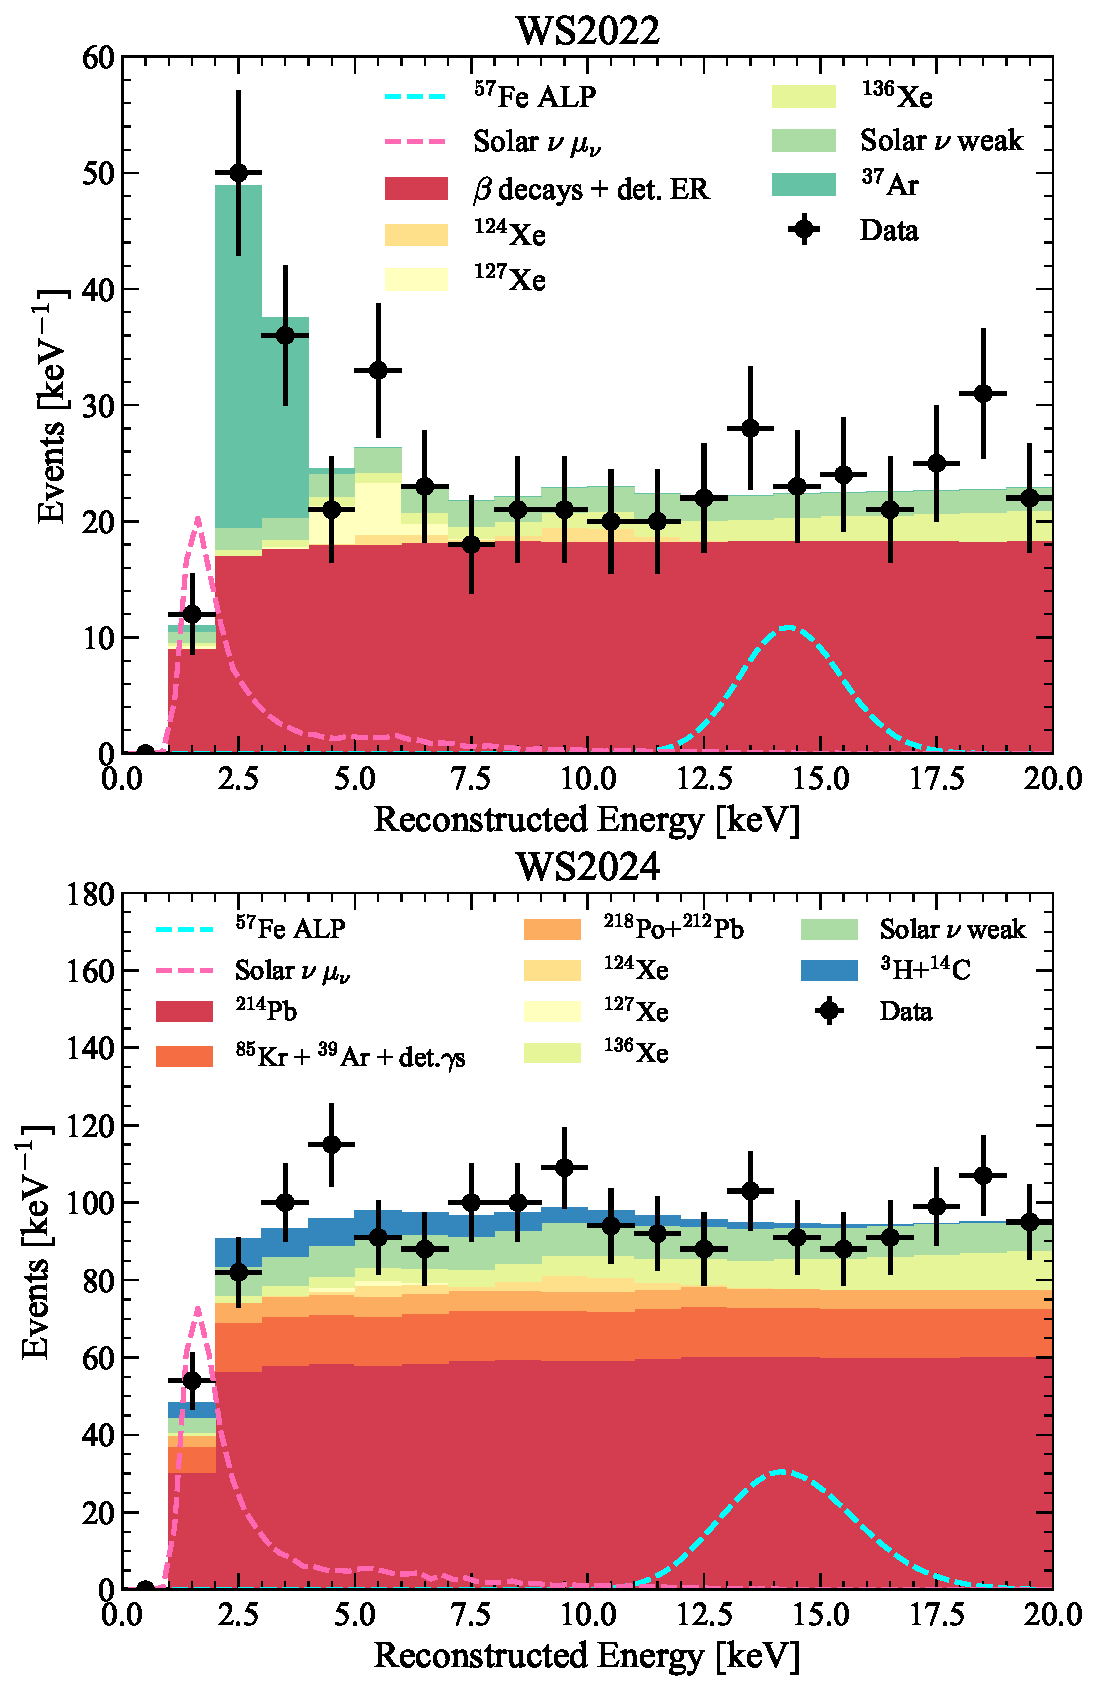
\includegraphics[width=0.47\linewidth, trim=0 0 0 14.3cm, clip]{DataPlot_bgfit.pdf} \\[4pt]
    \captionof{figure}{\small $\boldsymbol{^{85}}$Kr background contributions in XENONnT~\cite{XENON:2022ltv}~(left) and LZ~\cite{LZ:2025zpw}~(right) electronic-recoil searches.}
  \end{center}
  \vspace{16pt}

  The abundance of $\boldsymbol{^{85}}$Kr in $^{\mathrm{nat}}$Kr is taken to be $\boldsymbol{2\times10^{-11}}$~\cite{XENON:2022ltv}. Liquid-xenon dark matter experiments require $^{\mathrm{nat}}$Kr concentrations at the $\boldsymbol{\mathcal{O}}$(100)~ppq level, well below the ppb sensitivity typically achievable with commercially available measurement systems.
  \vspace{16pt}

  XENONnT removed $^{\mathrm{nat}}$Kr with the XENON1T cryogenic distillation system, while LZ used gas chromatography~\cite{XENON:2016bmq,Ames:2023lvd}. The residual concentrations were $\boldsymbol{(56 \pm 36)}$~ppq in XENONnT~\cite{XENON:2022ltv} (measured by gas chromatography--rare-gas mass spectrometry, GC-RGMS) and $\boldsymbol{(144 \pm 22)}$~ppq in LZ~\cite{LZ:2022ysc} (measured with a liquid-nitrogen~(LN$_2$) cold trap system developed by Prof.~Carter Hall's group at the University of Maryland, College Park).
  \vspace{16pt}

  At Columbia University, we are refurbishing the original krypton distillation columns from XENON100. To characterize their separation performance, we are developing a Maryland-style system, chosen for its simplicity, robustness, and potential portability.
\end{block}
\vspace{1.0cm}

\begin{block}{Methodology: Cold Trap + RGA}
  \begin{center}
    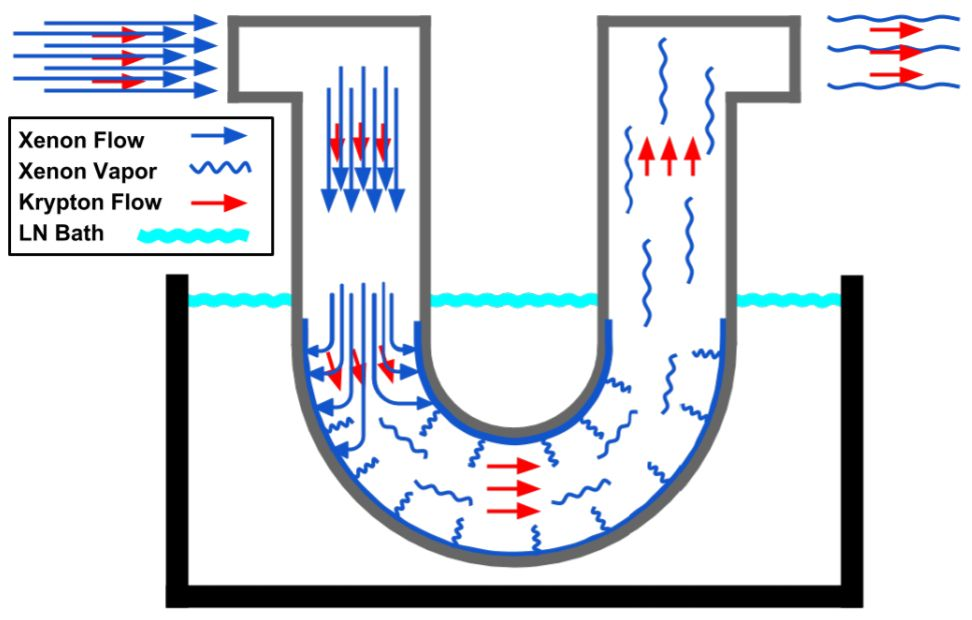
\includegraphics[width=0.9\linewidth]{schematic.jpg} \\[4pt]
    \captionof{figure}{\small Bulk Xe is frozen in an LN$_2$-cooled cold trap, enriching trace Kr in the gas phase~\cite{Armstrong:2025dhy}.}
  \end{center}
  \vspace{16pt}

  The measurement relies on the large difference between the vapor pressures of Xe and Kr at cryogenic temperature. As the Xe sample passes through the cold trap, bulk Xe freezes out while trace $^{\mathrm{nat}}$Kr remains preferentially in the gas phase. This suppresses the Xe load on the residual gas analyzer~(RGA) and effectively enriches the Kr concentration downstream.

  \vspace{16pt}
  The RGA then monitors the Kr partial pressure, which is converted to the $^{\mathrm{nat}}$Kr concentration in the original Xe sample referring to calibration. This cold-trap enrichment enables sensitivity far below commercial ppb-level gas analysis, targeting the $\mathcal{O}$(100)~ppq regime required by liquid-xenon dark matter experiments.
\end{block}
\vspace{1.0cm}

\end{column}

\hfill

% ============================================================
% RIGHT COLUMN
% ============================================================
\begin{column}{0.48\linewidth}

\begin{block}{\normalsize{XTRACT: Xenon Residual gas Analyzer with Cold Trap}}
  \begin{columns}
    \begin{column}{0.35\linewidth}
      \begin{center}
        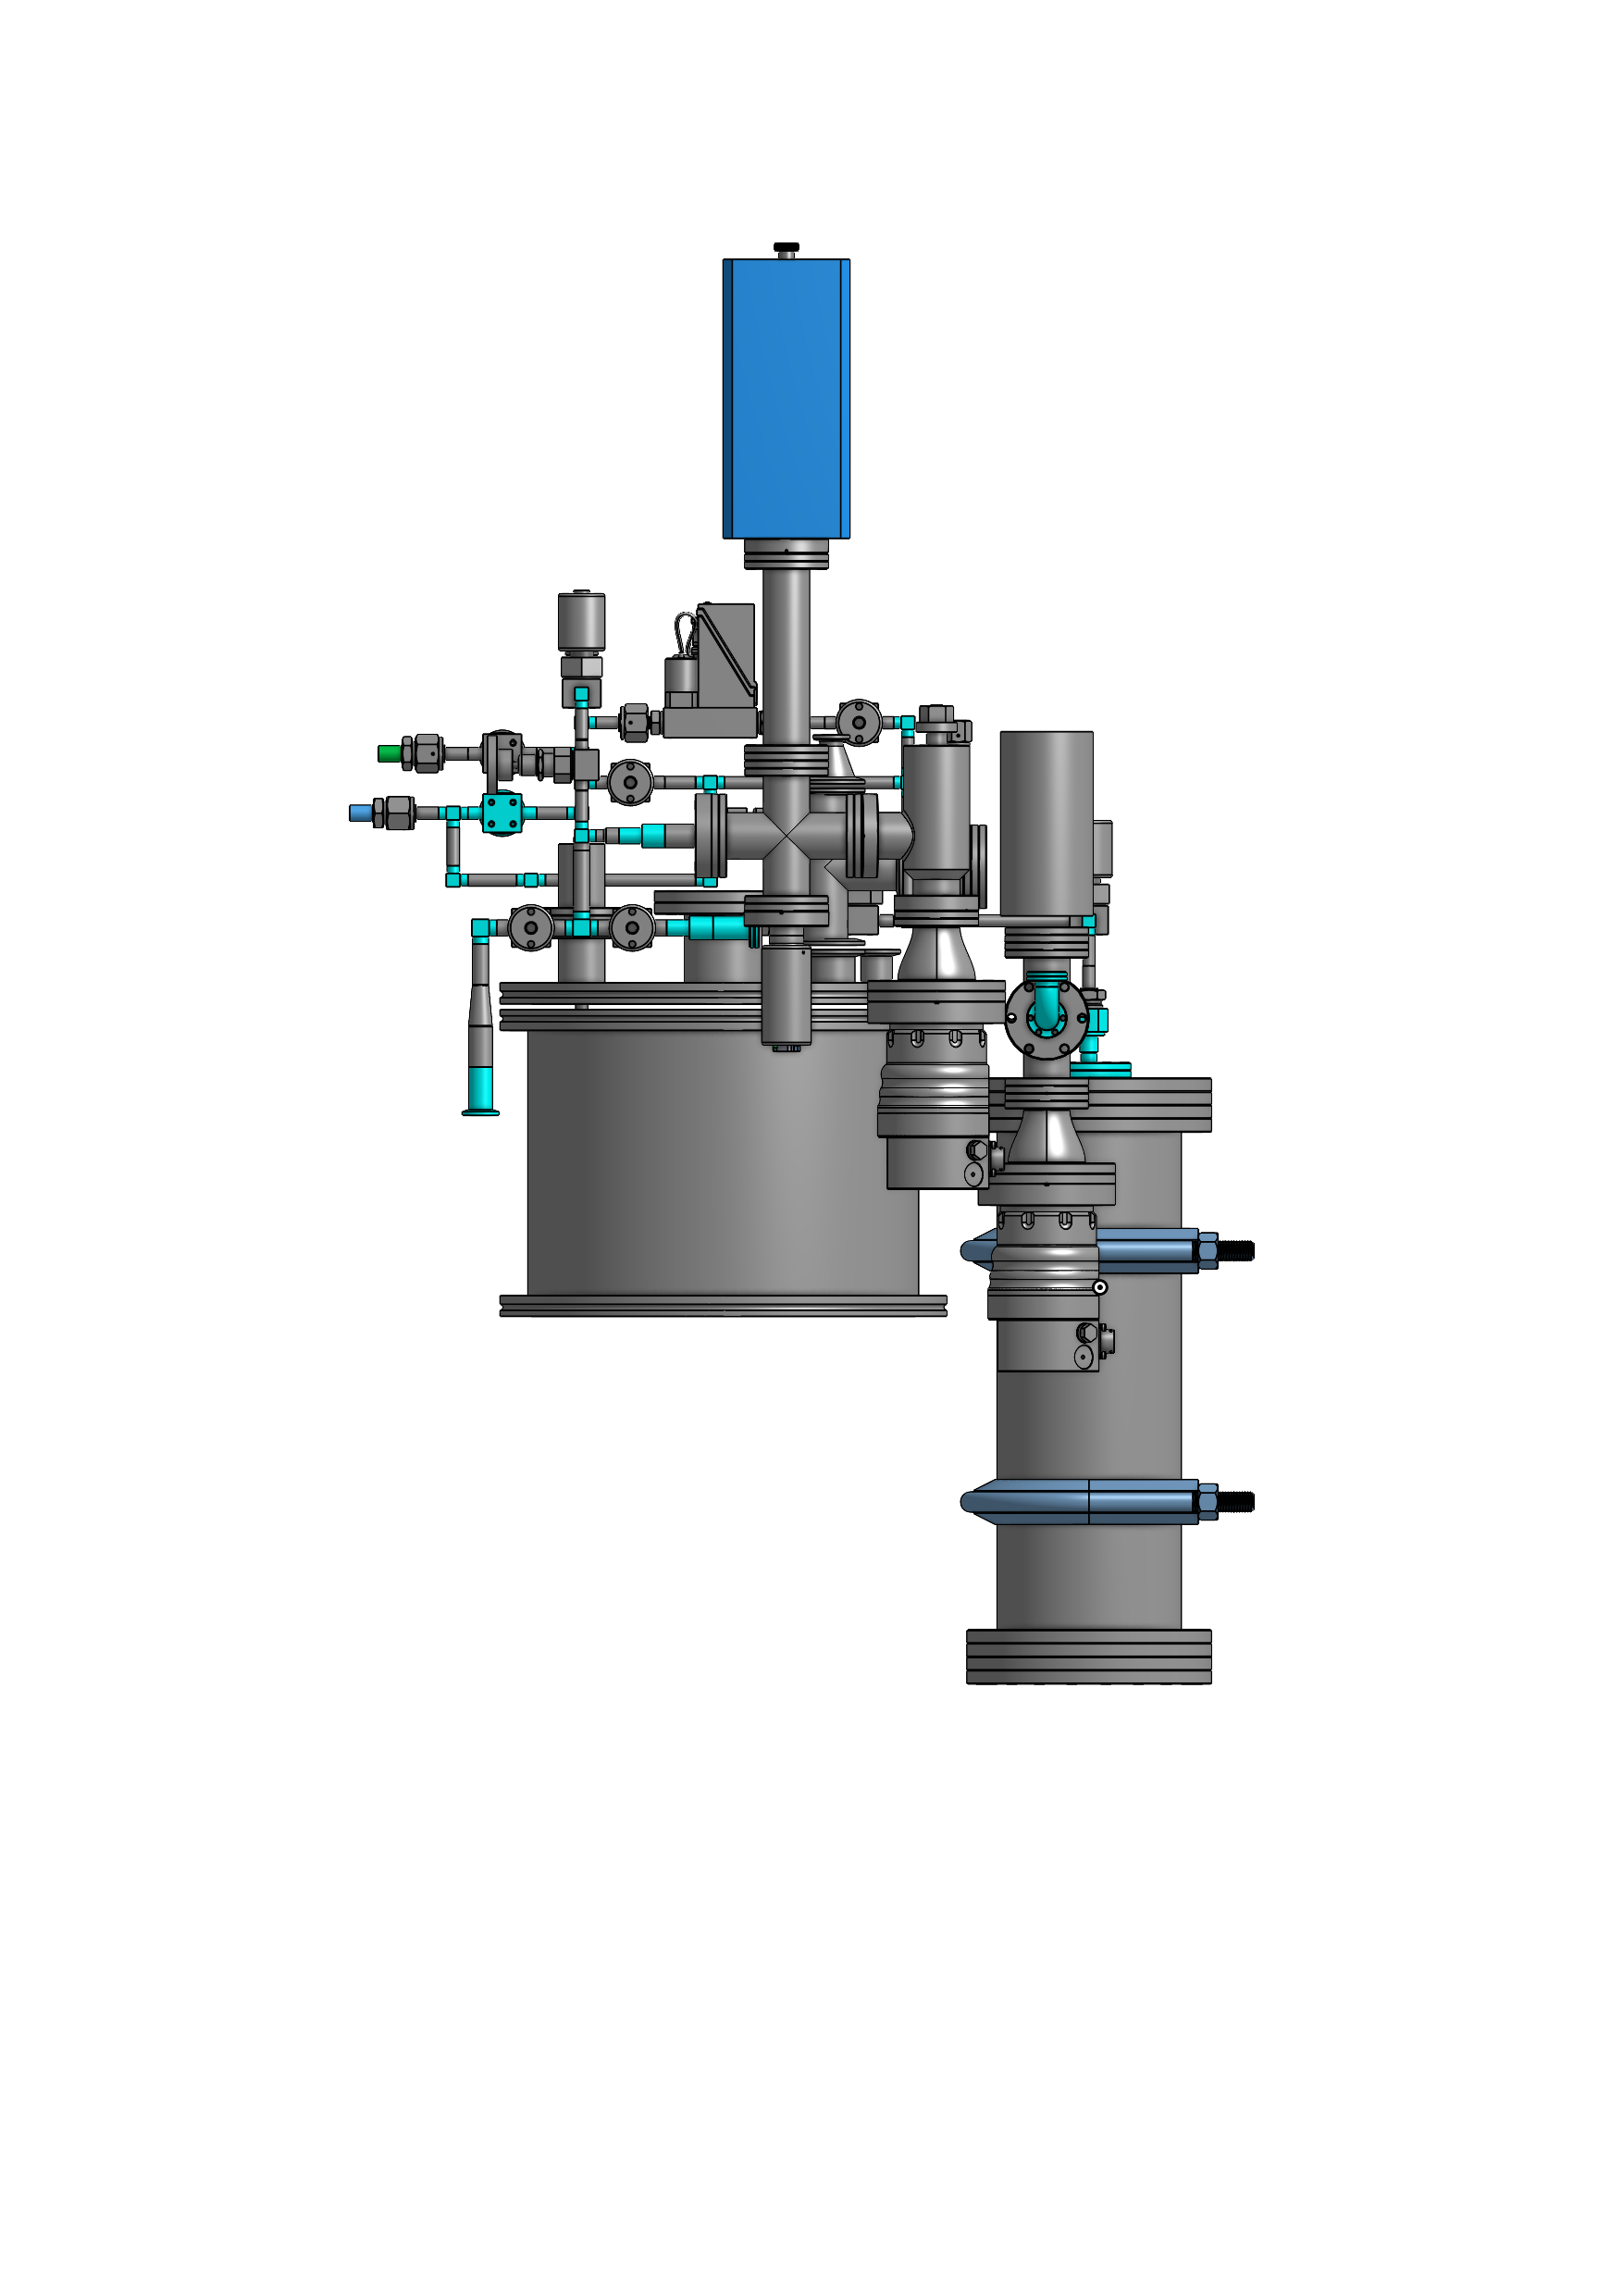
\includegraphics[width=0.7\linewidth, trim=5cm 9.5cm 7cm 4.5cm, clip]{XTRACT _ xtract-20260416_up.pdf} \\[4pt]
        \captionof{figure}{\small Side views of XTRACT; the support frame is omitted for clarity.}
      \end{center}
    \end{column}
    \begin{column}{0.65\linewidth}
      XTRACT adapts the Maryland-style cold trap design with several differentiations:
      \begin{itemize}
        \item Cryocooler-based operation, avoiding LN$_2$ handling and enabling continuous running.
        \item In-situ welded stainless-steel construction for leak tightness and reduced contamination; VCR fittings are used only at the main-volume interfaces.
        \item Compatibility with XENONnT and other liquid noble gas experiments, including potential underground deployment.
        \item Programmable logic controller~(PLC)-based automation for sample handling, cold trap operation, and RGA measurements.
      \end{itemize}

      The system uses only $\boldsymbol{\mathcal{O}}$(100)~g of xenon gas, with an estimated xenon loss below 1~g per measurement, negligible compared with the several-ton xenon inventory.
    \end{column}
  \end{columns}
\end{block}
\vspace{1.0cm}

\begin{alertblock}{Current Status \& Outlook}
  \begin{center}
    \includegraphics[width=0.7\linewidth]{IMG_7969.png} \\[4pt]
    \captionof{figure}{\small Assembled XTRACT system mounted on the aluminum support frame.}
  \end{center}

  \begin{itemize}
    \item[$\checkmark$] Designed and assembled a leak-tight system targeting $\mathcal{O}$(100)~ppq sensitivity for $^{\mathrm{nat}}$Kr measurements in xenon.
    \item[$\rightarrow$] Commissioning is underway with LN$_2$ cooling, followed by operation tests with a cryocooler.
    \item[$\rightarrow$] The mobile platform is being developed toward future integration with XENONnT and other liquid noble gas experiments.
  \end{itemize}
\end{alertblock}
\vspace{1.0cm}

\begin{block}{References}
  \scriptsize{\bibliographystyle{ieeetr}\bibliography{poster}}
\end{block}

\begin{columns}[T, totalwidth=\linewidth]
  \begin{column}{0.7\linewidth}
    \begin{block}{Acknowledgements}
      We gratefully acknowledge support from the National Science Foundation. We gratefully thank Prof.~Carter Hall and his group at the University of Maryland, College Park, especially Dr.~John Armstrong, for their guidance and for generously sharing their cold-trap design and expertise.
    \end{block}
  \end{column}
  \hfill
  \begin{column}{0.3\linewidth}
    \centering
    
\includegraphics[width=0.5\linewidth]{https_xenon_astro_columbia_edu_.pdf} \\[3pt]
    {\footnotesize The Aprile Group\\ at Columbia University}
  \end{column}
\end{columns}

\end{column}
\end{columns}

\end{frame}
\end{document}
